\section{A tree code with complementary traversals}
\label{sec:tree}

We use the affine label space $\mathcal A$ and row space
$H=\Aff(\mathcal A,\F)$ of \Cref{sec:preliminaries}.
The code below turns affine rows and Boolean gate tables into a word
indexed by labels. Its two complementary traversals control the
correlation seen by a cut that evaluates the word at a single label.

\begin{definition}[Tree code]
\label{def:tree-code}
Fix integers $s\ge2$ and $m\ge1$, and put
\[
 k=(2s)^m,\qquad d=s^m.
\]
Let $\mathcal T$ be the complete rooted $2s$-ary tree of depth $m$.
The children of each internal node $v$ are indexed by
$(g,b)\in[s]\times\{0,1\}$.  Its leaves are indexed by $[k]$.
To each internal node assign a table
$F_v:\F^s\to\{-1,1\}$, and to each leaf assign a row $R_i\in H$.
The word $W(R,F)\in\{-1,1\}^{\mathcal A}$ is defined pointwise as
follows.  At $a\in\mathcal A$, leaf $i$ has sign $(-1)^{R_i(a)}$.
An internal node with child signs $(Z_{g,b})$ outputs
\begin{equation}
 \left(\prod_{g=1}^s Z_{g,0}\right)F_v(z),
 \qquad (-1)^{z_g}=Z_{g,0}Z_{g,1}.
 \label{eq:gate-rule}
\end{equation}
The root output is $W(R,F)(a)$.
\end{definition}

We choose the tables to be noised by a second traversal of the tree.
A \emph{random slice} is obtained by first choosing
$J_0$ uniformly from $\{0,\ldots,m-1\}$.  Starting at the root,
at each reached node of depth less than $J_0$ choose one of its $s$
child pairs uniformly and independently, and continue through both
children of that pair.  The set $\mathcal D$ of reached nodes at
depth $J_0$ is the slice.

Conditionally on $J_0=j$, the slice has $2^j$ nodes, and every fixed
node of depth $j$ belongs to it with probability $s^{-j}$.
We write $F_{\rm out}=(F_u)_{u\notin\mathcal D}$ for the tables
outside the slice.

The two traversals of the tree used below complement one another.
The slice construction chooses one pair and keeps both children.
The Walsh expansion of a gate keeps one child from every pair.
Their intersection therefore follows a single path. Figure~\ref{fig:traversals}
shows the local rule; iterating it gives one common node at every slice depth.

\begin{figure}[ht]
\centering
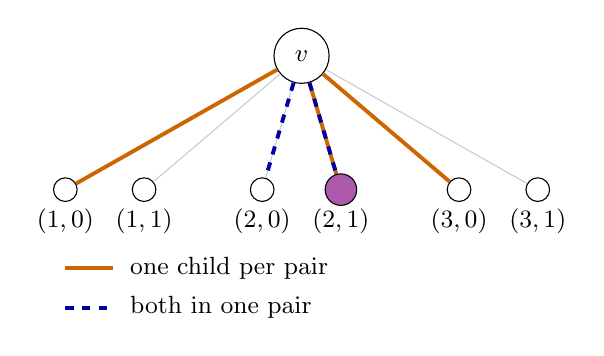
\begin{tikzpicture}[x=1cm,y=1cm,every node/.style={font=\small},
  mono/.style={draw=orange!80!black,line width=1.4pt},
  slice/.style={draw=blue!65!black,line width=1.4pt,dashed}]
\node[circle,draw,minimum size=7mm] (v) at (0,1.7) {$v$};
\foreach \x/\name/\lab in {-3/a/{(1,0)},-2/b/{(1,1)},-.5/c/{(2,0)},.5/d/{(2,1)},2/e/{(3,0)},3/f/{(3,1)}} {
 \node[circle,draw,fill=white,minimum size=3mm,inner sep=1pt] (\name) at (\x,0) {};
 \node[below] at (\x,-.12) {$\lab$};
 \draw[gray!40] (v) -- (\name);
}
\draw[mono] (v) -- (a);
\draw[mono] (v) -- (d);
\draw[mono] (v) -- (e);
\draw[slice] (v) -- (c);
\draw[slice] (v) -- (d);
\node[circle,draw,fill=violet!65,minimum size=4mm,inner sep=1pt] at (.5,0) {};
\draw[mono] (-3,-1) -- (-2.4,-1);
\node[anchor=west] at (-2.3,-1) {one child per pair};
\draw[slice] (-3,-1.5) -- (-2.4,-1.5);
\node[anchor=west] at (-2.3,-1.5) {both in one pair};
\end{tikzpicture}

\caption{Complementary choices at one gate, illustrated for $s=3$.
A monomial traversal (solid) selects one child from each pair; the slice
exploration (dashed) selects both children of one pair. Exactly one child
is shared, shown in purple. Only this local selection is depicted;
the same rule is repeated above the chosen slice.}
\label{fig:traversals}
\end{figure}

\begin{lemma}[Complementary traversal and correlation]
\label{lem:tree-correlation}
For every fixed collection of tables $F$, the root output as a
multilinear polynomial in the $k$ leaf signs has only degree-$d$
monomials.  Each such monomial chooses one child from every pair
at every node that it reaches.  Every resulting traversal meets
every possible slice $\mathcal D$ at exactly one node.
Consequently, negating all the tables on a slice negates $W$.

Let $0<t<1$ and $0<r<1$.  Draw $F$ uniformly, and construct $F'$
by leaving the tables outside $\mathcal D$ unchanged and coupling
each pair of corresponding table entries on $\mathcal D$ as
uniform signs of correlation $t$, independently across entries.
Independently draw
$R\in H^k$ uniformly, and form $R^1,R^2$ by retaining each row of
$R$ with probability $r$ and otherwise replacing it by an
independent uniform row, independently in the two copies.
Then, for every $a\in\mathcal A$ and every fixed slice,
\begin{equation}
 \E\bigl[W(R^1,F)(a)W(R^2,F')(a)\mid\mathcal D\bigr]
       =t r^{2d}.
 \label{eq:tree-correlation}
\end{equation}
In particular, if $r=1-\mu/d$ with $0<\mu<1/2$, then
$r^{2d}\ge1-2\mu$.
\end{lemma}

\begin{proof}
For a fixed gate table, expand in its argument $z$:
$F_v(z)=\sum_{I\subseteq[s]}\widehat F_v(I)(-1)^{\sum_{g\in I}z_g}$.
Substituting into Equation~\eqref{eq:gate-rule}, the term indexed
by $I$ is
\[
 \widehat F_v(I)
 \prod_{g\notin I}Z_{g,0}\prod_{g\in I}Z_{g,1}.
\]
Iterating this expansion gives
\begin{equation}
 W_F(x)=\sum_{P\in\mathscr P}a_P(F)\prod_{i\in P}x_i,
 \qquad |P|=d,
 \label{eq:tree-polynomial}
\end{equation}
where $\mathscr P$ is the family of leaf sets produced by choosing
one child per pair at each reached internal node.  The leaf set
determines all these choices: a selected child has a nonempty
intersection with that leaf set, whereas an unselected child has
none.  Thus different traversals give different monomials, and
$a_P(F)$ is the product of one Walsh coefficient of $F_v$ for each
node reached by the traversal.

At the root both a monomial traversal and the slice exploration
are present.  At any common node above the slice depth, exactly
one child is selected by both explorations.  Induction gives
exactly one common node at the slice depth.  Hence each $a_P$
contains exactly one factor from a table on $\mathcal D$.
Negating every such table negates each coefficient in
Equation~\eqref{eq:tree-polynomial} and therefore negates the word.
Moreover, each Walsh coefficient of a slice table satisfies
\[
 \E[\widehat F'_v(I)\mid F_v]=t\widehat F_v(I).
\]
Conditional independence between tables therefore gives
$\E[a_P(F')\mid F,\mathcal D]=t a_P(F)$.

For fixed $a$, the signs
$x_i^b=(-1)^{R_i^b(a)}$ are uniform, independent across $i$, and
$\E[x_i^1x_i^2]=r^2$.  Thus the product expectation of two
monomials in Equation~\eqref{eq:tree-polynomial} is zero unless
their leaf sets agree, and is $r^{2d}$ when they agree.
Since $W_F$ is Boolean, Parseval gives $\sum_P a_P(F)^2=1$.
Averaging first over rows and then over $F'$ proves
Equation~\eqref{eq:tree-correlation}.  The last claim is
Bernoulli's inequality:
$(1-\mu/d)^{2d}\ge1-2\mu$.
\end{proof}

The correlation identity describes a cut that evaluates the word at
one label. To analyze arbitrary cuts, we also need functions that can
depend on the entire word but do not see its generating rows or tables.
We call $f$ a \emph{function of the code} if
\begin{equation}
 f(R,F)=\phi(W(R,F))
 \label{eq:function-of-code}
\end{equation}
for a fixed function $\phi$ on words.  This class is closed under
averaging over fixed choices of $\phi$, including choices that
first pull a word back through a fixed affine map.
For $r\in[0,1]$, let $T_r$ denote independent row resampling with
retention probability $r$, and write $\bar f=T_rf$.
The operator preserves bounds on the range of $f$.
If $\phi$ is odd, Lemma~\ref{lem:tree-correlation} shows that both
$f$ and $\bar f$ are odd under simultaneous negation of the slice
tables.  In particular, they have mean zero in those table entries
when all rows and outside tables are fixed.

At these fixed data, the remaining random input is the cube of
$|\mathcal D|2^s$ independent entries, indexed by
$(v,z)\in\mathcal D\times\F^s$. Fourier degree and influence on this
cube refer to subsets of \emph{entries}. This differs from the Walsh
expansion of a fixed gate in its $s$-bit argument $z$ used in the
correlation proof.
